\documentclass[letter]{article}

\usepackage{amssymb, amsmath, amsthm, amsopn}
\usepackage{xspace}

\usepackage{graphicx}
\usepackage{xcolor}
\usepackage{tikz}
\usetikzlibrary{shapes,shapes.geometric,arrows,fit,calc,positioning,automata,shadows,patterns,backgrounds,
	decorations.pathreplacing,shapes.multipart,tikzmark, matrix}



\begin{document}
	\section{Logistic regression}
	
	Parameters used in logistic regression :
	\vspace{0.5cm}
	 
	\begin{tabular}{ccl}
		$n_x$ & : &  number of features \\
		$x\in\mathbb{R}^{n_x}$ & : & input features vector \\
		$y\in\{0,1\}$ & : & training label \\
		$w\in\mathbb{R}^{n_x}$ & : & weights \\
		$b\in\mathbb{R}$ & : & threshold \\
		$\hat{y} = \sigma(w^T x + b)$ & : & the output \\
		$\sigma(z) = \frac{1}{1+\exp(-z)}$ & : & sigmoid function
	\end{tabular}

	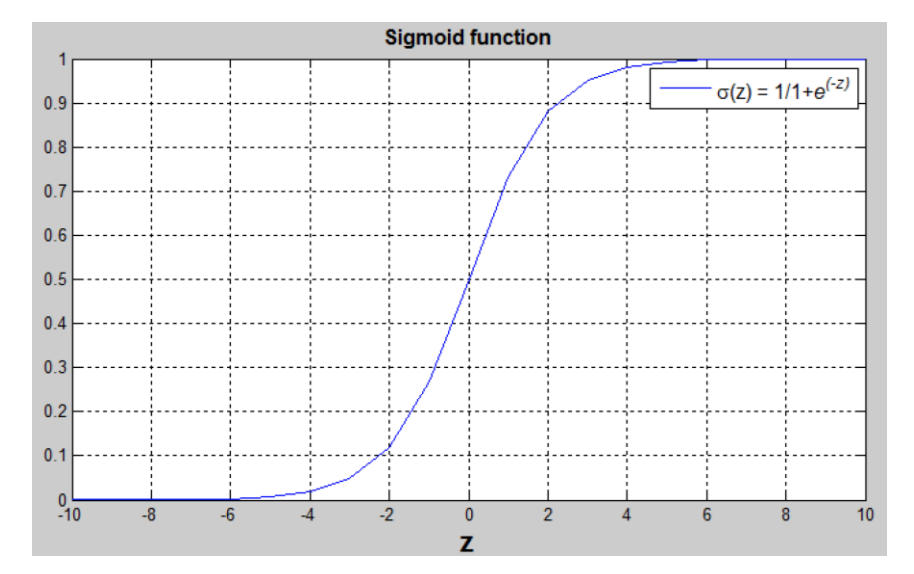
\includegraphics[scale=0.7]{sigmoid_function.png}
	
	
	\section{Neural Network}
	\begin{figure}
		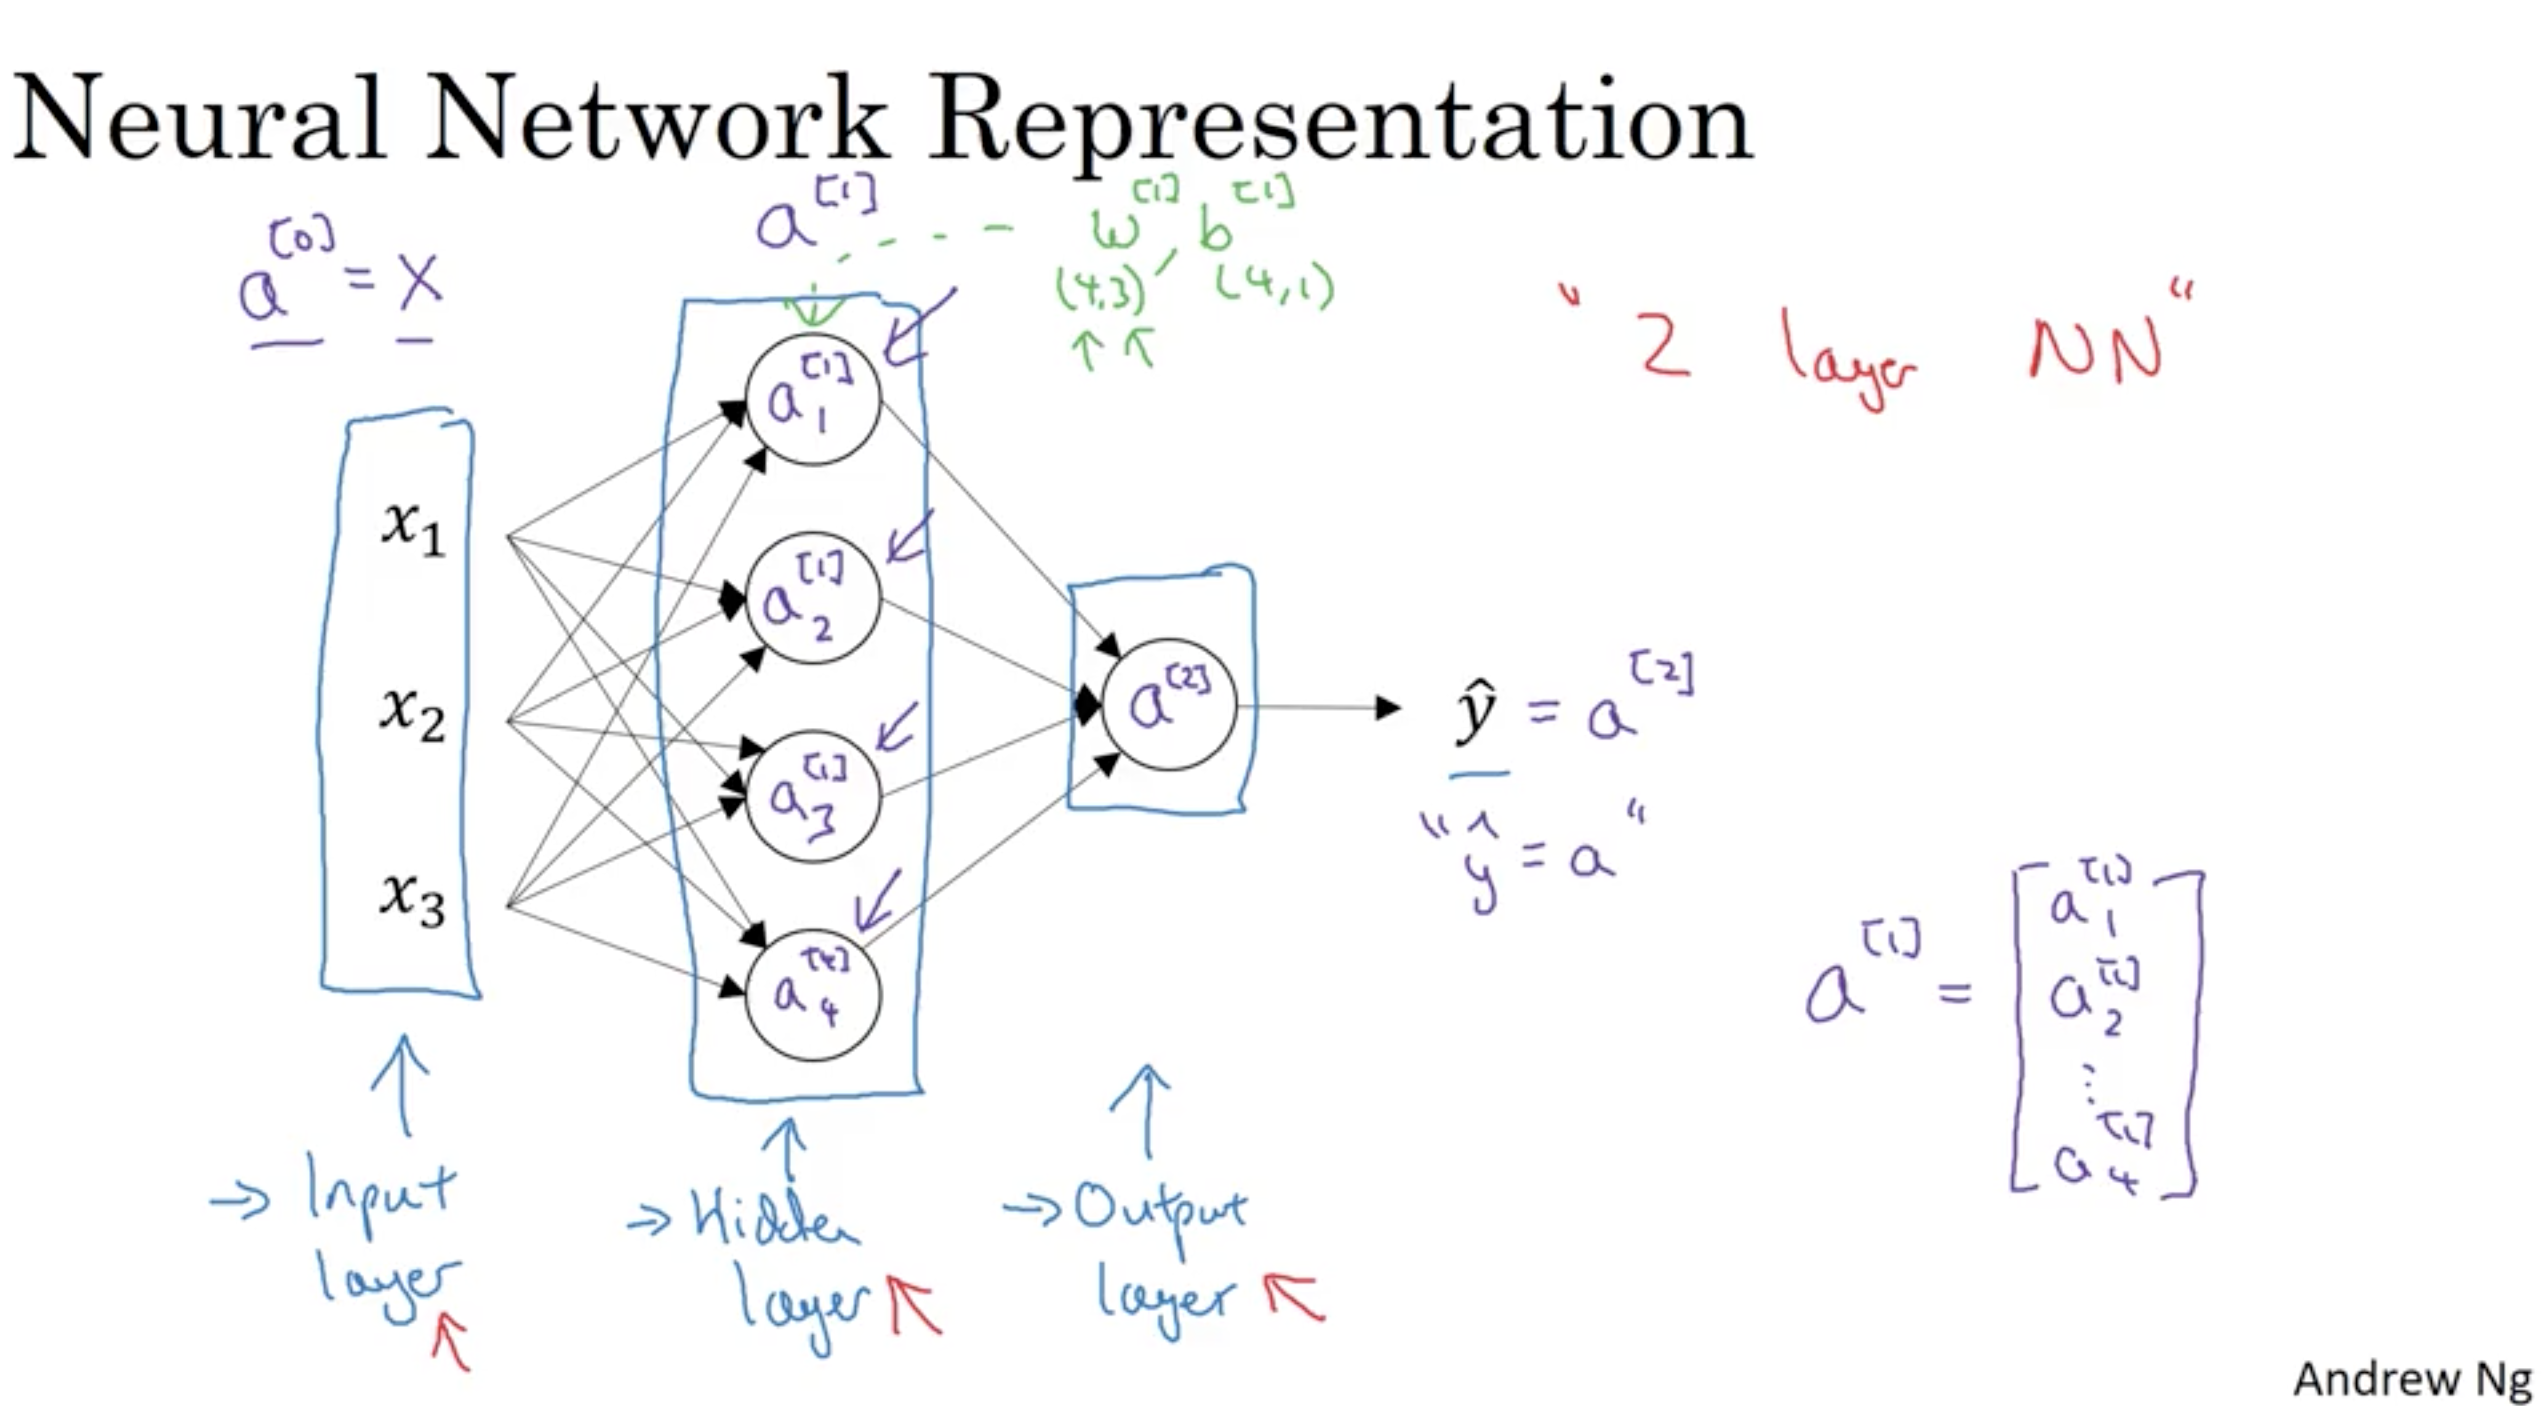
\includegraphics[scale=0.3]{neural_network_representation.png}
		\caption{
			Each node of the neural network corresponds to a different logistic regression computation.
			For example, $a_1^{[1]} = [w_{11}^{[1]}, w_{12}^{[1]}, w_{13}^{[1]}] \times [x_1, x_2, x_3]^T + b_1^{[1]}$.
		}
	\end{figure}
	
	
	
	
	
	
\end{document}